\section{L-systémy}\label{sec:L-systemy}

Uvedeme tuto kapitolu s~ohledem na předchozí obsah trochu netradičně a~od matematiky se (alespoň zdánlivě) na chvíli odkloníme. Podíváme se na fraktály, s jejichž způsobem popisu přišel roku 1968 maďarský biolog \name{Aristid Lindenmayer}\footnote{1925--1989}, a~který (možná pro někoho i~překvapivě) má základy především v~informatice. \citep[str. 2]{Prusinkiewicz1990}

K popisu specifického druhu fraktálů lze využít znalosti z~\emph{teorie formálních jazyků} a~\emph{teorie automatů}, na jejímž počátku stál (mj.) britský matematik a~informatik \name{Alan Turing}\footnote{1912--1954}. Ten ve svém článku \emph{On Computable Numbers, with an Application to the Entscheidungsproblem} z~roku 1936 zavedl koncept abstraktního stroje, dnes známého jako \emph{Turingův stroj}\index{Turingův stroj}\index{stroj!Turingův}. Jedná se o~jednoduché zařízení s~výpočetními schopnostmi již tehdy porovnatelnými se současnými počítači. Jeho princip fungování přitom není nikterak složitý. Pomineme-li nyní matematickou definici Turingova stroje, lze říci, že sestává ze tří hlavních částí:
\begin{enumerate}
    \item \textbf{Oboustranně nekonečná páska.} Páska je rozdělena na políčka, z nichž každé může obsahovat některý symbol z~předem známé abecedy (formálně vzato množiny) znaků.
    \item \textbf{Čtecí/zapisovací hlava.} Hlavu si můžeme představit jako čtecí/zapisovací "okénko", které stojí právě nad~jedním políčkem pásky. V~každém kroku stroj:
    \begin{itemize}
        \item přečte symbol pod~hlavou,
        \item podle svého stavu a~právě přečteného symbolu rozhodne, jakou akci provést.
    \end{itemize}
    \item \textbf{Řídicí jednotka.} Řídí chování stroje pomocí konečné množiny stavů
    \[Q=\set{q_0,q_1,\ldots,q_n}.\]
    Přechodová funkce $\delta$ pro (ne nutně všechny) dvojice $(\text{stav},\text{znak})$ udává:
    \begin{itemize}
        \item jaký symbol má hlava na pásku zapsat (může přepsat stávající symbol nebo nechat stejný),
        \item do jakého stavu se stroj přepne,
        \item jak se posune hlava: doleva (L), doprava (R) nebo zůstane (N).
    \end{itemize}    
\end{enumerate}
Výpočet pak probíhá takto:
\begin{enumerate}
    \item Stroj začíná ve stavu, který je stanovený jako počáteční. Na pásce je vložen vstup (řetězec symbolů), zbytek pásky je prázdný.
    \item Stroj vždy podle přechodové funkce stroje:
    \begin{itemize}
        \item přečte, co je pod~hlavou,
        \item zapíše (případně přepíše) symbol,
        \item přesune hlavu,
        \item přejde do dalšího stavu.
    \end{itemize}
    \item Pokud stroj nemá definovaný přechod pro aktuální stav a~čtený symbol na pásce, zastaví se. Pokud stroj skončil ve stavu, který je označený jako přijímající, pak stroj slovo \emph{přijal}, jinak jej \emph{odmítá}.
\end{enumerate}
Viz obrázek~\ref{fig:turinguv-stroj}.
\begin{figure}[h]
    \centering
    \includegraphics{ch04-turinguv-stroj.pdf}
    \caption{Znázornění Turingova stroje}
    \label{fig:turinguv-stroj}
\end{figure}
\begin{figure}[h]
    \centering
    \includegraphics[width=.4\textwidth]{Alan-Turing.jpeg}
    \caption[Alan Turing,~1912--1954]{Alan Turing,~1912--1954 (Převzato z~\cite{OConnorTuring2025})}
    \label{fig:alan-turing}
\end{figure}
V té době se Turing zabýval otázkou, kterou v~roce 1928 položil známý německý matematik \name{David Hilbert} (1862--1943). Je známá pod~názvem \emph{"Entscheidungsproblem"}\index{Entscheidungsproblem}\footnote{Anglicky \emph{The Decision problem}\index{The Decision problem}, česky přeložitelné jako \emph{"rozhodovací problém"}. Zde však poznamenejme, že onen český termín se používá i~v související teorii složitosti a~vyčíslitelnosti, má však podstatně jiný význam.}. Problémem bylo, zda existuje algoritmus, který o~každém matematickém tvrzení je schopný rozhodnout (v konečném čase), zda je, či není pravdivé. Později Alan Turing tento problém přeformuloval takto: \emph{Existuje program, který o~jiném programu na vstupu rozhodne, zda se zastaví, či nikoliv?} David Hilbert byl ve svých vizích optimistický, avšak nakonec Alan Turing dokázal, že \textbf{takový algoritmus nemůže existovat}. Způsob, jakým Turing došel k~onomu výsledku, byl v~konečném důsledku vlastně až překvapivě jednoduchý a~existuje pro něj velké množství popularizačních materiálů\footnote{Pokud by se chtěl čtenář dozvědět více o~této problematice a~teorii s~ní související, doporučujeme např. knihu \cite{Motwani2003}}.
\begin{figure}[h]
    \centering
    \includegraphics[width=.4\textwidth]{David-Hilbert.jpg}
    \caption[David Hilbert,~1862--1943]{David Hilbert,~1862--1943 (Převzato z~\cite{OConnorHilbert2025})}
    \label{fig:david-hilbert}
\end{figure}
Tím dal základ dnešní teoretické informatice. Turingův stroj, jakožto výpočetní model, stojí na samotném vrcholu hierarchie dalších výpočetních modelů\footnote{Mezi ně patří jmenovitě tzv. \textit{lineárně omezený automat}\index{automat!lineárně omezený}, \emph{zásobníkový automat}\index{automat!zásobníkový}, \emph{deterministický}\index{automat!deterministický} a~\emph{nedeterministický konečný automat}\index{automat!nedeterministický}.}, které jsou však svojí výpočetní silou slabší. Později pak americký lingvista \name{Noam Chomsky}\footnote{1928 až do současnosti (2025)} popsal celkem~4 základní třídy tzv. \emph{formálních jazyků}, které jsou dnes souhrnně známé pod~názvem \emph{Chomského hierarchie}\index{Chomského hierarchie}. Za formální jazyk považujeme určitou množinu slov (retězců). Chomského hierarchie zařazuje každý jazyk do jedné ze tříd podle typu tzv. \emph{formální gramatiky}, která slova z~daného jazyka generuje. O~gramatikách, a~obecně určitém základu teorie formálních jazyků, si ještě budeme podrobněji povídat. O~hlubší související teorii se čtenář může více dozvědět např. v~knize \cite{Motwani2003}.

\subsection{Stručně k~formálním jazykům a~gramatikám}\label{subsec:formalni-jazyky-a-gramatiky}

V úvodu této sekce jsme si již trochu přiblížili historické pozadí teorie formálních jazyků a~automatů (tou se již dále zabývat nebudeme, nicméně bylo by přinejmenším neslušné ji zde alespoň nezmínit vzhledem k~její přímé souvislosti s~touto problematikou). Ačkoliv tento text si neklade za cíl seznámit čtenáře se všemi podrobnostmi, byly zde zmíněny určité termíny, jejichž význam bude dobré si objasnit, konkrétně
\begin{itemize}
    \item \emph{formální jazyk}\index{formální!jazyk}\index{jazyk}
    \item a~\emph{formální gramatika}.\index{formální!gramatika}\index{gramatika}
\end{itemize}
\begin{definition}\label{def:formalni-jazyk-etc}
    Množinu symbolů (znaků)\index{symbol}\index{znak} $\Sigma$ nazýváme \emph{abeceda}\index{abeceda}.
    \begin{itemize}
        \item Libovolnou konečnou posloupnost znaků\index{znak}
        \[w=a_1a_2\ldots a_n,\]
        kde $a_i\in\Sigma$ pro každé $1\leqslant i\leqslant n$, nazýváme \emph{slovo}, popř. \emph{řetězec}.\index{slovo}\index{řetězec}
        \item Prázdným slovem\index{prázdné slovo} nazýváme slovo neobsahující žádné znaky, značíme ho $\lambda$.
        \item Délku slova\index{délka slova} $w$ značíme $|w|$, tzn.
        \[|w|=|a_1a_2\ldots a_n|=n.\]
        \item Množinu všech slov délky $n$ značíme $\Sigma^n$, tj.
        \[\Sigma^n=\set{a_1a_2\ldots a_n\mid a_i\in\Sigma\;\text{pro každé $i$}}.\]
        Speciálně $\Sigma^0=\set{\lambda}$.
        \item Množinu všech slov v~abecedě $\Sigma$ značíme $\Sigma^*$, tzn.
        \[\Sigma^*=\bigcup_{n=0}^\infty\Sigma^n.\]
        \item Množinu všech neprázdných slov v~abecedě $\Sigma$ značíme $\Sigma^+$, tzn.
        \[\Sigma^+=\Sigma^*\setminus\set{\lambda}.\]
        \item \emph{Formálním jazykem} (nebo zkráceně jen \emph{jazykem})\index{formální!jazyk}\index{jazyk} nazýváme libovolnou podmnožinu $L\subseteq\Sigma^*$.
    \end{itemize}
\end{definition}
\begin{example}
    Některé příklady abeced:
    \begin{itemize}
        \item $\Sigma=\set{0,1}$, tzv. \emph{binární abeceda}.
        \[\set{0,1}^*=\set{\lambda,0,1,00,01,10,11,000,001,\ldots}\]
        \item $\Sigma=\set{a,b,c,\ldots,z}$, tj. všechna písmena anglické abecedy.
        \[\set{a,b,c,\ldots,z}^*=\set{\lambda,a,b,c,\ldots,z,aa,ab,ac,\ldots}\]
        \item Všechny znaky ASCII\footnote{Zkratka pro \emph{American Standard Code for Information Interchange}. Stanovuje 128-bitové znakové kódování. Podotkněme, že ne všechny znaky jsou nutně tisknutelné a~mají čistě informativní charakter, avšak to nás zde z~formálního hladiska trápit vůbec nemusí.} tvoří abecedu.
    \end{itemize}
\end{example}
\begin{definition}[Operace se slovy]\label{def:operace-se-slovy}
    Nechť $\Sigma$ je libovolná abeceda a~mějme slova $u,v\in\Sigma^*$, kde $u=u_1u_2\ldots u_n$ a~$v=v_1v_2\ldots v_m$. Pak definujeme následující operace:
    \begin{itemize}
        \item \emph{Zřetězení (konkantenace)}\index{zřetězení}\index{konkantenace} slov $u$ a~$v$ je slovo
        \[uv=u_1u_2\ldots u_nv_1v_2\ldots v_m.\]
        Je celkem zjevné, že $|uv|=|u|+|v|=n+m$.
        \item Nechť $n\in\N$. Pak definujeme induktivně:
        \begin{align*}
            u^0&=\lambda,\\
            u^1&=u,\\
            u^n&=u^{n-1}u.
        \end{align*}
        Slovo $u^n$ se nazývá \emph{$n$-tá mocnina slova}\index{mocnina slova} $u$.
        \item \emph{Obráceným slovem $u$} rozumíme slovo $u^R=u_nu_{n-1}\ldots u_1$.
    \end{itemize}
\end{definition}
\begin{remark}
    Speciálně pro prázdné slovo $\lambda$ a~libovolné slovo $u\in\Sigma^*$ platí $u\lambda=\lambda u=u$.
\end{remark}
Na základě definice~\ref{def:operace-se-slovy} můžeme být nyní daleko konkrétnější při popisu některých slov a~jazyků. Např.
\[L=\set{0^n1^n\mid n\in\N_0}\]
značí jazyk všech slov obsahující znaky $0$ a~$1$ ve tvaru
\[\lambda,01,0011,000111,\ldots\]
O jazycích celkově lze dokázat řadu zajímavých tvrzení, která se přímo opírají o~již zmíněnou teorii automatů. V~tomto ohledu si dovolíme však hodně záležitostí přeskočit. Jazyky lze popisovat několika různými způsoby, avšak nás bude zajímat popis pomocí formálních gramatik\index{formální!gramatika}\index{gramatika}.
\begin{definition}[Formální gramatika]\label{def:formalni-gramatika}
    \emph{Formální gramatikou} (zkráceně jen \emph{gramatikou})\index{formální!gramatika}\index{gramatika} nazýváme uspořádanou čtveřici $G=(V,T,P,S)$, kde
    \begin{itemize}
        \item $V\neq\emptyset$ je množina \emph{neterminálů}\footnote{Anglicky \emph{variables}}\index{neterminál} (neterminálních symbolů)\index{neterminální symbol},
        \item $T\neq\emptyset$ je množina \emph{terminálů}\index{terminál} (terminálních symbolů)\index{terminální symbol},
        \item $S\in V$ je \emph{počáteční symbol},
        \item a~$P$ je množina přepisovacích \emph{pravidel}\footnote{Formálně vzato se jedná o~uspořádanou dvojici $(\alpha,\omega)$.}\index{přepisovací pravidlo}\index{pravidlo} ve tvaru $\beta A\gamma\to\omega$ (čteme "řetězec $\beta A\gamma$ se přepíše na řetezec $\omega$"), kde $A\in V$ a~$\beta,\gamma,\omega\in(V\cup T)^*$. Tzn.~levá strana každého pravidla obsahuje alespoň jeden neterminál.
    \end{itemize}
\end{definition}
\begin{definition}[Odvození slova v~gramatice]\label{def:odvozeni-slova-v-gramatice}
    Mějme gramatiku $G=(V,T,P,S)$. Říkáme, že
    \begin{itemize}
        \item $\alpha$ se \emph{přímo přepíše} na $\omega$, píšeme $\alpha\Rightarrow_G\omega$ nebo jen $\alpha\Rightarrow\omega$, jestliže
        \[\exists\beta,\gamma,\eta,\nu\in(V\cup T)^*: \alpha=\eta\beta\nu,\omega=\eta\gamma\nu\land(\beta\to\gamma)\in P.\]
        \item $\alpha$ se \emph{přepíše} na $\omega$, píšeme $\alpha\Rightarrow_G^*\omega$ nebo jen $\alpha\Rightarrow^*\omega$, pokud
        \[\exists\beta_1,\beta_2,\ldots,\beta_n\in(V\cup T)^*:\alpha=\beta_1\Rightarrow\beta_2\Rightarrow\dots\Rightarrow\beta_n=\omega.\]
    \end{itemize}
    Posloupnost $\beta_1,\ldots,\beta_n$ takovou, že $\beta_1\Rightarrow\beta_2\Rightarrow\dots\Rightarrow\beta_n$ nazýváme odvozením\index{odvození slova}. Též říkáme, že gramatika $G$ generuje slovo $w$, pokud $S\Rightarrow^* w$.
\end{definition}
Terminální symboly gramatiky představují znaky koncové abecedy, nad níž uvažujeme výsledná slova. Neobsahuje-li tedy slovo na konci odvození žádný neterminál, jsme hotovi.

Formální gramatiky nám umožňují rekurzivní definici jazyka. Jinak řečeno popisuje, jak lze slova daného jazyka generovat. Pravidla z~množiny $P$ lze aplikovat v~libovolném pořadí.
\begin{remark}
    \begin{itemize}
        \item Typicky platí, že pro neterminály používáme velká písmena abecedy $A,B,\ldots,Z$ a~pro terminály naopak malá písmena $a,b,\ldots,z$. Pro slova (řetězce) budeme využívat buď malá písmena řecké abecedy, nebo malá písmena z~konce abecedy, tj. $\dots,w,y,x,z$.
        \item Pokud máme více pravidel ve tvaru $\alpha\to\omega_i$, tj. se shodnou levou stranou, pak pro jejich zápis volíme tuto kompaktnější variantu:
        \[\alpha\to\omega_1\mid\omega_2\mid\dots\mid\omega_n.\]
    \end{itemize}
\end{remark}
\begin{example}
    Jazyk všech palindromů nad~binární abecedou, tj.
    \[L_\text{pal}=\set{w\in\set{0,1}^*\mid w=w^R}\]
    lze generovat gramatikou $G=\set{\set{S},\set{0,1},P,S}$, přičemž $P$ obsahuje následující pravidla:
    \[S\to\lambda\mid 0\mid 1\mid 0S0\mid 1S1.\]
    Kupříkladu slovo $w=011110$ lze odvodit takto:
    \[S\Rightarrow 0S0\Rightarrow 01S10\Rightarrow011S110\Rightarrow011\lambda 110=011110.\]
\end{example}
Trochu praktičtěji zaměřený příklad nám poskytuje~\ref{ex:syntax-analyza}. Gramatiky se typicky využívají (vyjma fraktální geometrie) např. v~kompilátorech\index{kompilátor} různých programovacích jazyků v~rámci tzv. \emph{syntaktické analýzy}\index{syntaktická analýza}, při níž se (jak název napovídá) kontroluje syntaktická správnost zápisu programu. Konkrétně se pro jednoduchost zaměříme pouze na matematické výrazy obsahující pouze operace \texttt{+} a~\texttt{*} (násobení).
\begin{example}\label{ex:syntax-analyza}
    Mějme gramatiku $G=(V,T,P,S)$, kde
    \[V=\set{E,I},T=\set{a,b,(,),+,*},S=E\]
    a~pravidla jsou následující:
    \begin{align*}
        E&\to I\mid E+E\mid E*E\mid (E)\\
        I&\to a\mid b\mid Ia\mid Ib.
    \end{align*}
    V~takto definované gramatice lze vygenerovat např. slovo
    \[w=(a+b)+bb*(ab+bb)\]
    následovně:
    \begin{align*}
        E&\Rightarrow E+E\Rightarrow(E)+E\Rightarrow(E)+E*E\Rightarrow(E)+E*(E)\\
        &\Rightarrow(E+E)+E*(E)\Rightarrow(E+E)+E*(E+E)\\
        &\Rightarrow^*(I+I)+I*(I+I)\Rightarrow^*(a+b)+Ib*(Ib+Ib)\\
        &\Rightarrow^*(a+b)+bb*(ab+bb).
    \end{align*}
\end{example}
S podobným přístupem se lze setkat i~např. v~lingvistice. Čtenář si možná ze základní školy vzpomíná na větný rozbor, v jehož rámci bylo úkolem určit pro zadanou větu její strukturu. Ve skutečnosti se nejedná o~nic jiného, než využití určité formální gramatiky $G=(V,T,P,S)$, jejíž pravidla v~množině $P$ jsou dána gramatickými pravidly (nyní v~lingvistickém slova smyslu) českého jazyka. Pro příklad viz obrázek\footnote{S, NP, VP, ADJP představují neterminály příslušné gramatiky a~jednotlivá slova (Petr, četl, pěknou, knihu) její terminály. Významy: S~\emph{(Sentence)}, NP \emph{(Noun Phrase)}, VP \emph{(Verb Phrase)}, ADJP \emph{(Adjective Phrase)}.}~\ref{fig:syntax-strom-vety}.
\begin{figure}[h]
    \centering
    \begin{tikzpicture}[
        edge from parent/.style={draw,-latex},
        level distance=1.5cm,
        sibling distance=3cm
      ]
        \node {S}
          child { node {NP}
            child { node {Petr} }
          }
          child { node {VP}
            child { node {\textit{četl}} }
            child { node {NP}
              child { node {ADJP}
                child { node {\textit{pěknou}} }
              }
              child { node {knihu} }
            }
          };
    \end{tikzpicture}
    \caption{Příklad syntaktického stromu věty: \emph{"Petr četl pěknou knihu."}}
    \label{fig:syntax-strom-vety}
\end{figure}
Zároveň zde můžeme vidět souvislost formální gramatiky s~gramatikou v~lingvistice.

\subsection{Definice L-systému}\label{subsec:definice-lsystemu}

V podsekci~\ref{subsec:formalni-jazyky-a-gramatiky} jsme v~podstatě viděli "rychloúvod" do problematiky \emph{formálních jazyků} a~\emph{gramatik}, kde jsme si především zavedli potřebnou terminologii a~značení. L-systémy\footnote{Pojmenovány po Aristidu Lindenmayerovi.}\index{L-systém} se v~kontextu formálních gramatik mírně, avšak podstatně, liší v~tom, že pravidla jsou v~jednom kroku aplikována paralelně.

Základní idea vychází z~konceptu, který jsme si již představili v~úvodní kapitole~\ref{chapter:uvod_do_fraktalu}, a to \emph{soběpodobnosti}\index{soběpodobnost}. V~každém dalším kroku jsme část útvaru nahradili jeho zmenšenou kopií. Nešlo by toto nějak zachytit pomocí postupného přepisování, jako tomu bylo v~případě formálních gramatik? Ovšem, že ano. Jako první se tedy podíváme na definici L-systému.
\begin{definition}[L-systém]\label{def:lsystem}
    L-systémem\index{L-systém} nazveme uspořádanou trojici $G=(V,\omega,P)$, kde:
    \begin{itemize}
        \item $V$ je abeceda,
        \item $\omega\in\Sigma^+$ je počáteční slovo zvané \emph{axiom}\index{axiom},
        \item a~$P$ je množina pravidel tvaru $a\to\alpha$, kde $a\in V$ a~$\alpha\in V^*$.
        \item Pro každé $a\in V$ platí $(a\to a)\in P$, pokud $a$ není na levé straně žádného jiného pravidla.
    \end{itemize}
\end{definition}
Porovnejme na chvíli definici~\ref{def:lsystem} s~definicí formální gramatiky uvedenou výše (viz definice~\ref{def:formalni-gramatika}). U~gramatik jsme rozlišovali tzv. neterminální a~terminální symboly. U~L-systému však tato dvojice druhů symbolů splývá, resp. nerozlišujeme mezi terminály a~neterminály, neboť v tomto případě nebude účelem generovat slova nějakého konkrétního jazyka (tj. nemá ani smysl rozlišovat, které symboly jsou součástí koncové abecedy). Dále začínáme rovnou s~řetězcem symbolů $\omega\in V^+$. To lze v~gramatice zařídit jednoduše tak, že zavedeme speciální neterminál $T$, který uvedeme jako počáteční, a~pak přidáme pravidlo $T\to\omega$, přičemž $\omega$, ani žádná jiná pravidla neobsahují neterminál $T$. V~tomto ohledu tedy můžeme vidět, že L-systém je z~pohledu definice gramatiky pouze zvláštní případ.

Jak už bylo uvedeno na začátku této podsekce, podstatný rozdíl oproti gramatikám nastává ve způsobu přepisování, resp. odvozování slov (pro připomenutí viz definice~\ref{def:odvozeni-slova-v-gramatice}).
\begin{definition}[Odvození slova v~L-systému]\label{def:odvozeni-slova-v-lsystemu}
    Nechť je dán L-systém $G=(V,\omega,P)$.
    \begin{itemize}
        \item Slovo $\alpha=a_1a_2\ldots a_n\in V^+$, kde $a_i\in V$, se \emph{přímo přepíše} na $\omega=\omega_1\omega_2\ldots\omega_n$, kde $\omega_i\in V^*$ pro každé $1\leqslant i\leqslant n$, pokud
        \[\forall i\in\N,1\leqslant i\leqslant n: (a_i\to\omega_i)\in P.\]
        Píšeme $\alpha\Rightarrow_G\omega$ nebo jen $\alpha\Rightarrow\omega$.
        \item Slovo $\alpha$ se \emph{přepíše} na $\omega$, pokud
        \[\exists\beta_1,\beta_2,\ldots,\beta_n\in V^*:\alpha=\beta_1\Rightarrow\beta_2\Rightarrow\dots\Rightarrow\beta_n=\omega.\]
        Píšeme $\alpha\Rightarrow_G^*\omega$ neboj jen $\alpha\Rightarrow^*\omega$.
    \end{itemize}
\end{definition}
Zatím jsme se moc nepozastavili nad~poslední podmínkou v~definici~\ref{def:lsystem}. Zajišťuje nám, že každý znak lze vždy přepsat na jiný řetězec. Zkuste si schválně rozmyslet, že právě díky této podmínce dává definice odvození slova~\ref{def:odvozeni-slova-v-lsystemu} smysl.

Než se posuneme dál, zkusme se ještě věnovat různým variantám\linebreak L-systémů. Definice~\ref{def:lsystem}, kterou jsme si uvedli, ve skutečnosti odráží pouze jeden ze speciálních případů. Tomuto typu se říká \emph{bezkontextové}\index{bezkontextový L-systém} L-systémy (značené \emph{OL-systémy}\index{OL-systém}). Název vychází z~faktu, že každý symbol přepisujeme zvlášť (připouštíme pouze pravidla ve tvaru $a\to\omega$, kde $a\in V$ a~$\omega\in V^*$), tzn. nezáleží na ostatních znacích (tedy kontextu, v němž se nachází). Jinými typy L-systémů jsou naopak \emph{kontextové}\footnote{Tyto typy L-systémů souvisí do jisté míry s~již v~úvodu zmíněnou Chomského hierarchií\index{Chomského hierarchie}, v~jejímž rámci jsou definovány podobně i~bezkontextové a~kontextové gramatiky.}, u~nichž pracujeme s~pravidly ve tvaru $\gamma A\beta\to\gamma\omega\beta$, kde $\gamma,\beta,\omega\in V^*$ a~$A\in V$.

Dále lze L-systémy rozlišovat podle toho, zda pro každý řetězec $\alpha\in V^*$ existuje právě jedno pravidlo $\alpha\to\omega$, nebo existuje více pravidel v~$P$, které obsahují $\alpha$ na levé straně. Takový typům L-systémů se říká \emph{deterministické}\footnote{Tzn. je jednoznačně určeno, na jaký řetězec bude $\alpha$ přepsáno.}\index{L-systém!deterministický}\index{deterministický L-systém}, resp. \emph{nedeterministické}\index{L-systém!nedeterministický}\index{nedeterministický L-systém}. Pro deterministické bezkontextové L-systémy se pak užívá značení \emph{DOL-systémy}\index{DOL-systém}, což je i~případ, kterým se budeme dále zabývat. Pokud by čtenáře tato teorie zajímala více, doporučujeme knihu \cite{Prusinkiewicz1990}.

\subsection{Želví grafika}\label{subsec:zelvi-grafika}

Pro neznalého čtenáře se může zdát zarážející, že zde pracujeme celou dobu s~řetězci znaků a~nikoliv s~geometrickými útvary. Zde si ukážeme, jak interpretovat výsledné řetězce pomocí tzv. \emph{želví grafiky}\index{želví grafika}.

Představme, že máme virtuální želvu v~$\R^2$, jejíž stav reprezentujeme pomocí trojice $(x,y,\alpha)$, kde $(x,y)$ jsou její pozice\footnote{Situaci lze pochopitelně zobecnit do $\R^n$. Ve vyšších dimenzích bychom museli zavést symboly pro rotaci okolo každé osy zvlášť.} a~$\alpha$ je orientovaný úhel udávající její směr. Dále máme pevně zadanou délku kroku $d>0$ a~přírůstek úhlu $\delta$. Definujeme základní čtveřici symbolů, s níž budeme v~rámci abecedy $V$ pracovat. Symboly budou reprezentovat jednotlivé akce pro želvu. Jejich význam udává tabulka~\ref{table:vyznam-symbolu-zelva}.
\begin{table}[h]
    \centering
    \begin{tabular}{lp{0.8\textwidth}}
        $F$ & Želva se přesune o~vzdálenost $d$. Stav se změní na $(x^\prime,y^\prime,\alpha)$, kde $x^\prime=x+d\cos\alpha$ a~$y^\prime=y+d\sin\alpha$, a~zároveň je nakreslena úsečka mezi body $(x,y)$ a~$(x^\prime,y^\prime)$.\\
        $f$ & Želva se přesune o~vzdálenost $d$ bez kreslení úsečky.\\
        $+$ & Želva se otočí doleva o~úhel $\delta$. Nový stav bude $(x,y,\alpha+\delta)$.\\
        $-$ & Želva se otočí doprava o~úhel $\delta$. Nový stav bude $(x,y,\alpha-\delta)$.
    \end{tabular}
    \caption{Význam symbolů v~abecedě $V$ pro želvu}
    \label{table:vyznam-symbolu-zelva}
\end{table}

Pracujeme tedy v~základu s~abecedou $V=\set{F,f,+,-}$ (později dodefinujeme ještě další symboly). Předpokládáme, že počáteční stav želvy je vždy $(0,0,0)$. Začneme s~velice jednoduchou ukázkou, kde $\delta=\pi/6$ a~krok $d$ volíme libovolně. Pro začátek se podíváme na Kochovu křivku, kterou už jsme viděli v~sekci~\ref{sec:sobepodobnost}.
\begin{itemize}
    \item \emph{Axiom $\omega=F$}
    \item \emph{Pravidla $P$: $F\to F-F----F-F$}
\end{itemize}
Iterováním tohoto L-systému postupně dostaneme slova:
\begin{itemize}
    \item $n=0$: $F$
    \item $n=1$: $F-F----F-F$
    \item $n=2$: $F-F----F-F-F-F----F-F----F-F----F-F-F-F----F-F$
    \item $n=3$: $F-F----F-F-F-F----F-F----F-F----F-F-F-F----F-F-F-F----F-F-F-F----F-F----F-F----F-F-F-F----F-F----F-F----F-F-F-F----F-F----F-F----F-F-F-F----F-F-F-F----F-F-F-F----F-F----F-F----F-F-F-F----F-F$
\end{itemize}
Délka řetězce poroste exponenciálně\footnote{Podobná situace nastává pro ostatní fraktály, které si zde ještě představíme. Generování vyšších iterací daných útvarů je proto často výpočetně náročné.}. Výslednou interpretaci daných řetězců můžeme vidět na obrázku~\ref{fig:lsystem-kochova-krivka}.
\begin{figure}[h]
    \centering
    \includegraphics[scale=\fractalscale]{ch01-kochova-krivka-0iterace.pdf}
    \begin{center}
        $n=0$
    \end{center}
    \vspace{.5cm}
    \includegraphics[scale=\fractalscale]{ch01-kochova-krivka-1iterace.pdf}
    \begin{center}
        $n=1$
    \end{center}
    \vspace{.5cm}
    \includegraphics[scale=\fractalscale]{ch01-kochova-krivka-2iterace.pdf}
    \begin{center}
        $n=2$
    \end{center}
    \vspace{.5cm}
    \includegraphics[scale=\fractalscale]{ch01-kochova-krivka-3iterace.pdf}
    \begin{center}
        $n=3$
    \end{center}
    \caption{Interpretace vygenerovaných řetězců pro Kochovu křivku}
    \label{fig:lsystem-kochova-krivka}
\end{figure}
Všimněme si, že právě onen rekurzivní "charakter" gramatik, resp. L-systémů nám pomáhá dobře zachytit soběpodobnost (viz sekce~\ref{sec:sobepodobnost}) daných útvarů. Lindenmayer původně přišel s~L-systémy kvůli modelování růstu a~vývoje rostlin. Takový proces však není jednoduše popsatelný a~hraje při něm roli jistá míra náhody. \cite{Prusinkiewicz1990} I~takové případy lze modelovat\footnote{Konkrétně pomocí tzv. \emph{stochastických L-systémů}\index{stochastický L-systém}\index{L-systém!stochastický}, kde každému pravidlu přiřadíme pravděpodobnost aplikace v~dalším kroku.}. Pro zachování rozumného rozsahu tohoto textu se podíváme čistě na deterministické varianty. Na další typy fraktálů a~jejich L-systémů jsou uvedeny v~podsekci~\ref{subsec:ukazky-fraktalu-lsystemy}.

V případě modelování rostlin se nám hodí zavést ještě další dvojici symbolů. Mnohdy se nám stane, že se potřebujeme vrátit na určitou pozici, kde želva již stála. To by bylo možné vyřešit např. zpětným chodem želvy do původní pozice, nicméně velice špatně by se s~tímto pracovalo v~rámci L-systému. Proto si nejdříve vysvětlíme pojem tzv. \emph{zásobníku}\index{zásobník}.

Koncept zásobníku je programátorům nejspíše velmi dobře známý, nicméně pro "neprogramátory" si jej zde krátce vysvětlíme. Jedná se datovou strukturu pro dočasné ukládání dat, přičemž jeho charakteristikou je, že data, která jsou zařazena do zásobníku jako poslední jsou jako první odebrána. Pro tento způsob manipulace s~daty se používá zkratka \emph{LIFO\footnote{Alternativním způsobem je \emph{FIFO\index{FIFO} -- First In, First Out}, který je využíván u~tzv.\emph{fronty}\index{fronta}.}\index{LIFO} -- Last In, First Out}. V~rámci zásobníku máme dvojici základních operací:
\begin{itemize}
    \item \emph{vložení prvku na vrchol zásobníku} (tzv. operace \texttt{push}),~
    \item a~\emph{odebrání prvku z~vrcholu zásobníku} (tzv. operace \texttt{pop}).
\end{itemize}
Pro znázornění zásobníku viz obrázek~\ref{fig:zasobnik}. Do abecedy $V$ zavedeme nové znaky uvedené níže. 
\begin{table}[H]
    \centering
    \begin{tabular}{lp{0.8\textwidth}}
        $[$ & Uložení aktuálního stavu želvy $(x,y,\alpha)$ na zásobník.\\
        $]$ & Odebere stav uložený na vrcholu zásobníku a~nastaví jej jako aktuální stav želvy.
    \end{tabular}
    \caption{Význam symbolů v~abecedě $V$ pro želvu}
    \label{table:vyznam-symbolu-zelva-zasobnik}
\end{table}
Tato dvojice symbolů nám umožňuje využít želví grafiku pro vykreslení dalších fraktálních útvarů, neboť máme možnost si určitých místech ukládat stav želvy, k~němuž se lze posléze vrátit. Uvažujme např. L-systém definovaný takto (viz obrázek~\ref{fig:fraktalni-strom}):
\begin{itemize}
    \item \emph{Axiom:} $\omega=F$,
    \item \emph{Pravidla $P$:} $F\to FF-[-F+F+F]+[+F-F-F]$,
    \item $\delta=\pi/8$.
\end{itemize}
\newpage
\begin{figure}[H]
    \centering
    \begin{subfigure}{0.3\textwidth}
        \centering
        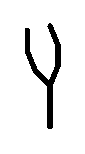
\includegraphics[width=0.3\textwidth]{bracketed-ol-1-iter1.pdf}
        \begin{center}
            $n=1$
        \end{center}
    \end{subfigure}
    \begin{subfigure}{0.3\textwidth}
        \centering
        \includegraphics[width=0.5\textwidth]{bracketed-ol-1-iter2.pdf}
        \begin{center}
            $n=2$
        \end{center}
    \end{subfigure}
    \begin{subfigure}{0.3\textwidth}
        \centering
        \includegraphics[width=0.9\textwidth]{bracketed-ol-1-iter3.pdf}
        \begin{center}
            $n=3$
        \end{center}
    \end{subfigure}
    \begin{subfigure}{0.6\textwidth}
        \centering
        \includegraphics[width=\textwidth]{bracketed-ol-1-iter4.pdf}
        \begin{center}
            $n=4$
        \end{center}
    \end{subfigure}
    \caption{Fraktální strom pro $n=1,2,3,4$}
    \label{fig:fraktalni-strom}
\end{figure}
\begin{figure}[H]
    \centering
    \includegraphics{ch04-zasobnik.pdf}
    \caption{Znázornění zásobníku}
    \label{fig:zasobnik}
\end{figure}

\subsection{Ukázky fraktálů a~jejich L-systémů}\label{subsec:ukazky-fraktalu-lsystemy}

Zde lze nalézt některé další ukázky fraktálů a~jejich L-systémů. Všechny obrázky fraktálních útvarů, které jste zde viděli a~ještě uvidíte jsou vygenerovány pomocí programu\footnote{viz odkaz na GitHub repozitář: \url{https://github.com/D4vEOFF/Py-Fractal-Generator}} přiloženého k~tomuto textu. Všechny tyto příklady jsou převaty z~knihy \cite{Prusinkiewicz1990}, kde lze též nalézt mnoho dalších.

Zároveň zde ještě dodejme, že někdy se též můžeme setkat se situací, kdy potřebujeme více než jeden neterminál, tedy kromě $F$ máme ještě jiné znaky. Obecně však platí, že jejich interpretace v~želví grafice je stejná jako pro symbol $F$.
\begin{figure}[p]
    \centering
    \includegraphics[width=0.4\textwidth]{koch-curve-1-iter0.pdf}\qquad
    
\includegraphics[width=0.4\textwidth]{koch-curve-1-iter1.pdf}\qquad\\
    \includegraphics[width=0.4\textwidth]{koch-curve-1-iter2.pdf}\qquad
    \includegraphics[width=0.4\textwidth]{koch-curve-1-iter3.pdf}\qquad\\
    \includegraphics[width=0.4\textwidth]{koch-curve-1-iter4.pdf}\qquad
    \begin{align*}
        \omega&=F-F-F-F\\
        F&\to FF-F-F-F-FF\\
        \delta&=\pi/2
    \end{align*}
    \caption{Varianta Kochovy křivky}
    \label{fig:lsystem-varianta-kochovy-krivky}
\end{figure}
\begin{figure}[p]
    \centering
    \includegraphics[width=0.4\textwidth]{lakes-and-islands-iter0.pdf}\qquad
    \includegraphics[width=0.4\textwidth]{lakes-and-islands-iter1.pdf}\qquad\\
    \includegraphics[width=0.6\textwidth]{lakes-and-islands-iter2.pdf}
    \begin{align*}
        \omega&=F+F+F+F\\
        F&\to F+f-FF+F+FF+Ff+FF-f+FF-F-FF-Ff-FFF\\
        f&\to ffffff\\
        \delta&=\pi/2
    \end{align*}
    \caption{Jezera a~ostrovy}
    \label{fig:lsystem-jezera-a-ostrovy}
\end{figure}
\begin{figure}[H]
    \centering
    \includegraphics[width=0.4\textwidth]{fass-curve-1.pdf}
    \begin{align*}
        \omega&=L\\
        L&\to L+R++R-L--LL-R+\\
        R&\to -L+RR++R+L--L-R\\
        \delta&=\pi/3\\
        n&=4
    \end{align*}
    \caption{Prostor vyplňující křivka}
    \label{fig:prostor-vyplnujici-krivka}
\end{figure}
% \begin{figure}[H]
%     \centering
%     \begin{subfigure}{0.45\textwidth}
%         \centering
%         \includegraphics[width=0.6\textwidth]{bracketed-ol-2-iter4.pdf}
%         \begin{align*}
%             \omega&=F\\
%             F&\to F[+F]F[-F]F\\
%             \delta&=25{,}7^\circ\\
%             n&=4
%         \end{align*}
%     \end{subfigure}
%     \qquad
%     \begin{subfigure}{0.45\textwidth}
%         \centering
%         \includegraphics[width=0.7\textwidth]{bracketed-ol-3-iter5.pdf}
%         \begin{align*}
%             \omega&=X\\
%             X&\to F[+X][-X]FX\\
%             F&\to FF\\
%             \delta&=25{,}7^\circ\\
%             n&=5
%         \end{align*}
%     \end{subfigure}
%     \caption{Fraktální stromy I~a II}
%     \label{fig:lsystem-fraktalni-strom-i-ii}
% \end{figure}
\begin{figure}[p]
    \centering
    \includegraphics[height=0.8\textheight]{bracketed-ol-2-iter4.pdf}
    \begin{align*}
        \omega&=F\\
        F&\to F[+F]F[-F]F\\
        \delta&=25{,}7^\circ\\
        n&=4
    \end{align*}
    \caption{Fraktální strom I}
    \label{fig:lsystem-fraktalni-strom-i}
\end{figure}
\begin{figure}[p]
    \centering
    \includegraphics[height=0.8\textheight]{bracketed-ol-3-iter5.pdf}
    \begin{align*}
        \omega&=X\\
        X&\to F[+X][-X]FX\\
        F&\to FF\\
        \delta&=25{,}7^\circ\\
        n&=4
    \end{align*}
    \caption{Fraktální strom II}
    \label{fig:lsystem-fraktalni-strom-ii}
\end{figure}
\begin{figure}[p]
    \centering
    \includegraphics[width=0.8\textwidth]{bracketed-ol-4-iter5.pdf}
    \begin{align*}
        \omega&=X\\
        X&\to F-[[X]+X]+F[+FX]-X\\
        F&\to FF\\
        \delta&=22{,}5^\circ\\
        n&=5
    \end{align*}
    \caption{Fraktální strom III}
    \label{fig:lsystem-fraktalni-strom-iii}
\end{figure}
\begin{figure}[H]
    \centering
    \includegraphics[width=0.8\textwidth]{sierpinsky-triangle-lsystem-iter8.pdf}
    \begin{align*}
        \omega&=A\\
        A&\to B-A-B\\
        B&\to A+B+A\\
        \delta&=\pi/3\\
        n&=8
    \end{align*}
    \caption{L-systém pro Sierpińského trojúhelník}
    \label{fig:lsystem-sierpinskeho-trojúhelnik}
\end{figure}